\chapter{Исследовательский раздел}
\label{cha:research}
    \par В данном разделе приведено описание планирования экспериментов и их результаты.
    \section{Технические характеристики}

    \par Технические характеристики машины, на которой выполнялось исследование:
    \begin{itemize}
        \item операционная система: macOS Ventura 13.0; [\ref{bib:11}]
        \item оперативная память: 8 Gb;
        \item процессор: Apple M1. [\ref{bib:12}]
    \end{itemize}

    \section{Постановка исследования}
    \par Целью эксперимента является определение зависимости времени генерации изображения модели планетарной системы в зависимости от количества точек, аппроксимирующих поверхности объектов сцены. Количество точек для всех объектов является одинаковым. Эксперимент проводится при параметрах сетки (см \ref{cha:research}), принимающих значение от 0 до 20.
    \par Во время тестирования устройство было подключено к блоку питания и не нагружено никакими приложениями, кроме встроенных приложений окружения, окружением и системой тестирования. Оптимизация компилятора была отключена.
    \par По результатам эксперимента составляется сравнительная таблица, а также строится график зависимостей.

    \section{Результат эксперимента}
    \par В таблице \ref{table:gen} приведены результаты эксперимента. На рисунке (\ref{schema:graph}) представлены результаты эксперимента в графическом виде. 

        \begin{table}[h!]
            \caption{Зависимость процессорного времени генерации изображения от кол-ва точек}
            \centering
            \begin{tabular}{|r|r|r|}
            \hline
            Кол-во точек & Параметр сетки & Время (мс)  \\\hline
            10 & 0 & 0.000 \\ \hline
            53 & 1 & 1.659 \\ \hline
            127 & 2 & 4.272 \\ \hline
            233 & 3 & 7.564 \\ \hline
            371 & 4 & 13.761 \\ \hline
            541 & 5 & 26.961 \\ \hline
            743 & 6 & 42.740 \\ \hline
            977 & 7 & 72.107 \\ \hline
            1243 & 8 & 97.179 \\ \hline
            1541 & 9 & 159.422 \\ \hline
            1871 & 10 & 199.826 \\ \hline
            2233 & 11 & 283.439 \\ \hline
            2627 & 12 & 363.550 \\ \hline
            3053 & 13 & 459.466 \\ \hline
            3511 & 14 & 627.598 \\ \hline
            4001 & 15 & 823.686 \\ \hline
            4523 & 16 & 1041.410 \\ \hline{}
            5077 & 17 & 1278.590 \\ \hline
            5663 & 18 & 1590.800 \\ \hline
            6281 & 19 & 1956.390 \\ \hline
            6931 & 20 & 2414.680 \\ \hline
            \end{tabular}
            \label{table:gen}
        \end{table}

    \begin{figure}[h!]
        \centering
        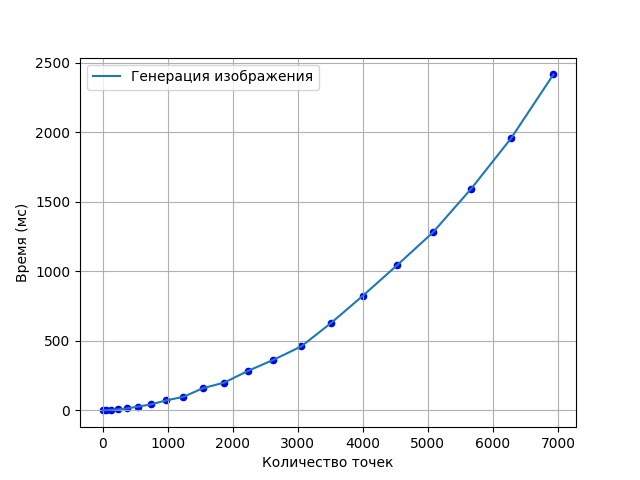
\includegraphics[scale=0.8]{inc/graph.png}
        \caption{Зависимость замеренного времени генерации изображения от кол-ва точек объекта}
        \label{schema:graph}
    \end{figure}\clearpage
    \par Так как \begin{math} \log_{\frac{6931}{53}}{\frac{2414}{1}} \approx 1.598\end{math}, то зависимость стремится к квадратичной.
    \section{Выводы из исследовательсного раздела}
    \par По результатам исследования можно сделать вывод, что время генерации изображения зависит от количества точек, аппроксимирующих поверхности объектов, причем зависимость стремится к квадратичной.
\newpage